\documentclass[]{beamer}
\usepackage[utf8]{inputenc}
\usepackage[T1]{fontenc}
\usepackage{default}
\usepackage[ngerman]{babel}

\usepackage{datetime}

%\usepackage{caption,subcaption}
\usepackage{natbib}

% \usepackage{overpic}
\usepackage{floatflt}
\usepackage{tikz}
\usepackage{pgf}
\usepackage{bm}

\usepackage{array}
\usepackage{booktabs}
\usepackage{enumerate}

\usepackage{amsmath}
\usepackage{listings}
\lstset{language=Python,numbers=left,escapeinside={[}{]}}

\usepackage{graphicx}

\usepackage{todonotes}
\presetkeys{todonotes}{inline,size=\tiny}{}

\makeatletter
\newenvironment{myitemize}{%
   \setlength{\topsep}{0pt}
   \setlength{\partopsep}{0pt}
   \renewcommand*{\@listi}{\leftmargin\leftmargini \parsep\z@ \topsep\z@ \itemsep\z@}
   \let\@listI\@listi
   \itemize
}{\enditemize}
\makeatother

\newcommand{\executeIfFileNewer}[3]{%
  \ifnum\pdfstrcmp{\pdffilemoddate{#1}}{\pdffilemoddate{#2}} > 0%
    \immediate\write18{#3}%
  \fi%
}

\graphicspath{{figures/pdf/},{figures/}}

\newcommand{\inputSVG} [2][]{%
  \executeIfFileNewer{figures/#2.svg}{figures/pdf/#2.pdf}{%
    inkscape -z -D --file=figures/#2.svg --export-pdf=figures/pdf/#2.pdf --export-latex --export-area-drawing}%
  #1%
  \input{figures/pdf/#2.pdf_tex}%
}

\usetheme{Antibes}
\usecolortheme{dolphin}

\setbeamercovered{transparent}
\beamertemplatenavigationsymbolsempty
\setbeamertemplate{footline}[frame number]

% \setbeamercolor{title}{fg=red!80!black,bg=red!20!white}

\usefonttheme[onlylarge]{structuresmallcapsserif}
\usefonttheme[onlysmall]{structurebold}

\title{Meine Privatsphäre im Internet}

\author[T. Bopst, S. Köhler]{Thomas Bopst, Steffen Köhler}
\newdateformat{writtenDate}{\THEDAY. \monthname[\THEMONTH]~\THEYEAR} % d. MONAT yyyy
\date{\writtenDate\formatdate{18}{12}{2014}}

\begin{document}
\bibliographystyle{apalike}

\frame{\titlepage}

\section*{Fragen}

\setbeamercovered{invisible}
\begin{frame}
  \frametitle{Fragen}

  \begin{itemize}
   \item Wer sorgt sich um die eigene Privatsphäre?
   \pause
   \item Hast du ein Problem damit, dass Andere deine Textnachrichten mitlesen?
   \pause
   \item Was für Maßnahmen unternehmt ihr um eure Textnachrichten zu schützen?
   \pause
   \item Wer würde seine Nachrichten gerne schützen, weiß jedoch nicht wie?
  \end{itemize}

\end{frame}



\frame{%
  \frametitle{Inhaltsverzeichnis}
  \tableofcontents
}

\section{Einleitung}

\begin{frame}
  \frametitle{Motivation}

  Ziele:
  \begin{itemize}
   \item Bewusstsein für Privatsphäre im digitalen Raum schaffen
   \item Möglichkeiten zum Schutz der Privatsphäre aufzeigen
  \end{itemize}

  \vspace{2ex}

  Was wir nicht wollen:
  \begin{itemize}
    \item Eine Musterlösung vorgeben!
    \item Missionieren
  \end{itemize}
\end{frame}


\section{Deine Spuren im Netz}

\begin{frame}
\frametitle{Was ist ein Cookie?}

\begin{itemize}
  \item Identifikationsnummer, die vom Anbieter vergeben wird
  \item Verwendet um BesucherInnen wiederzuerkennen
\note{Notwendig für Sessions}
  \item Werden im Web-Browser gespeichert
\note{IE, Firefox, Safari ...}
  \item Werden in der Regel nicht automatisch gelöscht
  \item $\rightarrow$ bspw. kein erneuter Login notwendig
\note{Google, Facebook, GMX, ...}
\end{itemize}

\end{frame}

\begin{frame}
\frametitle{Profilbildung im Netz}

\begin{itemize}
  \item Like (Facebook), +1 (Google), Tweet (Twitter), \dots
  \item Über Cookies mit persönlichem Profil verknüpfbar
\note{ggf. werden Daten an dritte weitergegeben (Versicherungen etc)}
\note{personalisierte Werbung}
\note{TODO Bild Hänsel und Gretel mit Cookiespur}
\end{itemize}

\end{frame}

\begin{frame}
  \frametitle{Wie schütze ich mich davor}
  \begin{itemize}
    \item Cookies löschen?
    \item Ghostery, etc.
   \note{Disconnect, TrackMeNot}
    \item Adblocker
    \item DuckDuckGo
   \note{Cookies von Werbeanbietern}
  \end{itemize}
\end{frame}


% Überleitung zu Instantmessaging, da ja noch viel schlimmer.

\section{Instant Messaging}

\frame{
  \frametitle{Inhaltsverzeichnis}
  \tableofcontents[currentsection]
}

\begin{frame}
  \frametitle{Übertragungsweg von Nachrichten}
  %\todo[inline]{Schaubild Übertragung von Nachrichten (über Server)}
  \center \inputSVG[\def\svgscale{0.25}]{Orange_blue_message_transportation_de}
  \note{Analogie: Brief/Postkarte mit Adresse}
\end{frame}

\begin{frame}
  \frametitle{Symmetrische Verschlüsselung}
  \begin{columns}[c]
    \begin{column}{0.5\textwidth}
      \center \inputSVG[\def\svgscale{0.2}]{Orange_blue_symmetric_cryptography_de}
    \end{column}
  \end{columns}
  %\todo[inline]{Schaubild Verschlüsselung (symm)}
\end{frame}

\begin{frame}
  \frametitle{Transportwegverschlüsselung / Ende-zu-Ende Verschlüsselung}
  Transportwegverschlüsselung
  \begin{center}
    \inputSVG[\def\svgscale{0.25}]{Orange_blue_message_transportation_security_de}
  \end{center}


  Ende-zu-Ende Verschlüsselung
  \center \inputSVG[\def\svgscale{0.25}]{Orange_blue_message_end_to_end_de}
%  \todo[inline]{Schaubild vgl. Ende-zu-Ende / Transportweg}
\end{frame}

\begin{frame}
  \frametitle{Transportweg- und Ende-zu-Ende Verschlüsselung}
  \todo[inline]{Ende-zu-Ende + Transportweg}
\end{frame}

\begin{frame}
  \frametitle{Open Source vs. Closed Source}
  \begin{definition}[Open Source]
   Programm mit öffentlich zugänglichem Quellcode \hfill \tiny [Duden]
  \end{definition}

  \begin{itemize}
   \item Programm kann von jedem geprüft werden
   \item Schwer Hintertüren einzubauen
   \item Notwenige Bedingung für prüfbar sichere Programme
   \item Open Source $\neq$ kostenlos
  \end{itemize}

\end{frame}


\begin{frame}
  \frametitle{EFF Scorecard zu Messaging Apps}
  \center
  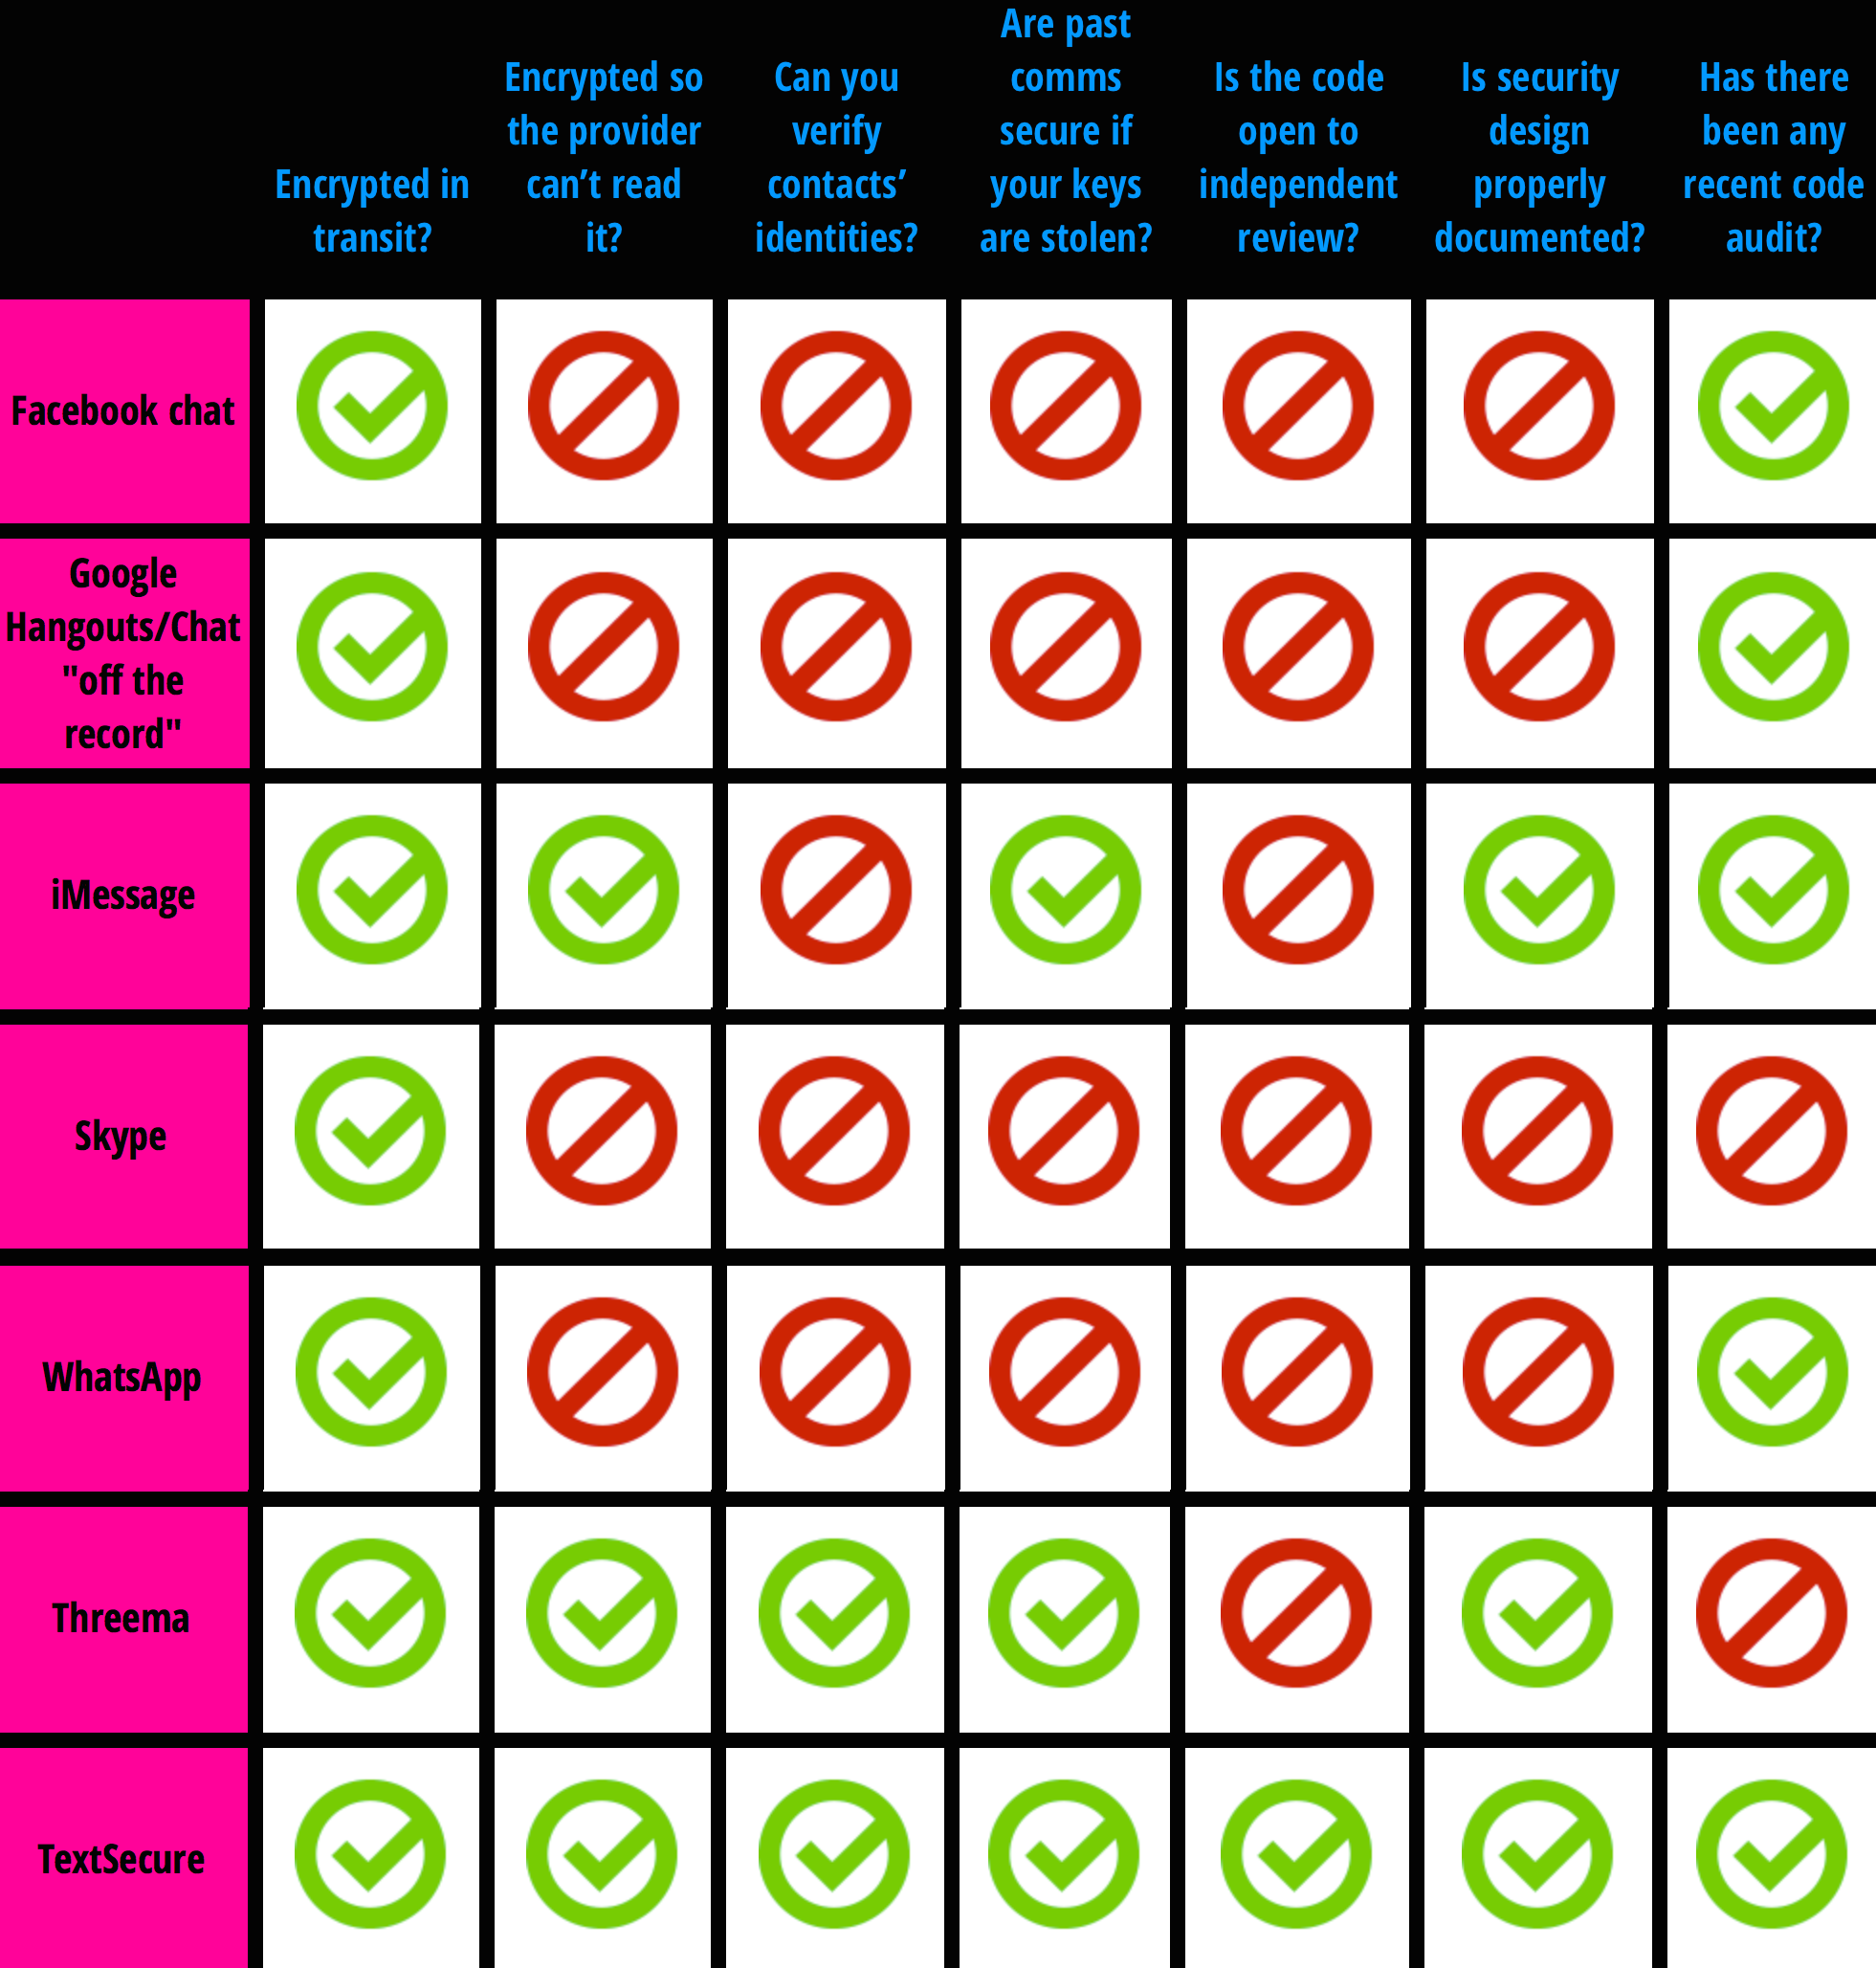
\includegraphics[width=0.6\textwidth]{figures/eff_scorecard.png}
\end{frame}

\begin{frame}
  \frametitle{Identitätsprüfung}
  \todo[inline]{Screenshots}
\end{frame}

\section{E-Mail Verschlüsselung}

\begin{frame}
  \frametitle{Probleme symmetrischer Verschlüsselung}
  \begin{itemize}
    \item Verteilung der Schlüssel
    \item Anzahl benötigter Schlüssel
    \begin{itemize}
      \item 2 Personen $\rightarrow$ 1 Schlüssel
      \item 3 Personen $\rightarrow$ 3 Schlüssel
      \item 4 Personen $\rightarrow$ 6 Schlüssel
      \item 100 Personen $\rightarrow$ 4950 Schlüssel
      \item n Personen $\rightarrow$ $\frac{n(n-1)}{2}$ Schlüssel
    \end{itemize}
    \todo[inline]{Evtl auf Tafel rechnen}
    \todo[inline]{Graph}
  \end{itemize}

\end{frame}

\begin{frame}
   \frametitle{Asymmetrische Verschlüsselung}
   
   \todo[inline]{Schaubild}
\end{frame}

\begin{frame}
  \frametitle{Schlüsselserver (Keyserver)}
  \todo[inline]{Schaubild}
\end{frame}

\begin{frame}
  \frametitle{Identitätsprüfung}
  \begin{itemize}
    \item Keine Echtheitsgarantie für Schlüssel auf Schlüsselserver
    \item ``Web of Trust''
    \note{Schlüssel nur signieren wenn WIRKLICH geprüft}
  \end{itemize}
  \todo[inline]{Schaubild (ger. graph)}
\end{frame}

\begin{frame}
  \frametitle{Signaturen}
  \todo[inline]{Schaubild Signaturschema}
  \todo[inline]{Schaubild Signatur generieren + prüfen mit pub/sec key}
\end{frame}

\begin{frame}
  \frametitle{Signierte E-Mail}
  \begin{itemize}
    \item Garantiert Echtheit des Absenders
    \item Keine Verschlüsselung!
    \note{Unterschriebener Vertrag}
    \item Kann aber mit Verschlüsselung kombiniert werden
  \end{itemize}
\end{frame}

%\section{Quellen}

%\begin{frame}
%  \nocite{*}
%  \tiny
%  \frametitle{Quellen}
%  \bibliography{references}
%\end{frame}

\end{document}
